\section{Invariance par rotation et symétrie}
\subsection{Redressement de la main}
\subsubsection{Présentation de la méthode}
Un des premiers problèmes que nous avons rencontré est lié à la rotation des mains, certaines mains ne sont pas orientées verticalement alors que nos classifieurs font l'hypothèse que toutes les mains sont orientées verticalement (c'est à dire avec les doigts vers le haut). Pour redresser la main, il nous fallait tout d'abord déterminer la direction de la main dans l'image. Pour ceci, nous avons utilisé une technique inspirée de l'analyse en composantes principales pour estimer la direction "principale" de l'image.

Soit $I$ une image segmentée et binarisée d'une main, définissons $P$ l'ensemble des positions des pixels appartenant à la main dans $I$. Nous déterminons alors la matrice de covariance de ces points par rapport à leur centre de gravité (qui correspond à la valeur moyenne des points), et nous considérons les $2$ vecteurs propres de cette matrice. Nous considérons que l'un d'entre eux est la direction de la main (\autoref{fig:pca}). Nous appliquons alors une rotation à l'image segmentée binarisée de façon à obtenir la verticale dans la direction de ce vecteur propre. Le calcul a été implémentée à l'aide de la classe PCA d'OpenCV.

\subsubsection{Analyse}
Cette méthode a 2 défauts:
\begin{itemize}
\item La direction donnée pointe parfois vers le poignet au lieu des doigts. Ce problème peut être résolu par une méthode invariante par rotation d'angle $\pi$, comme l'histogramme radial.
\item La méthode donne de mauvais résultats lorsqu'aucun doigt n'est levé.
\end{itemize}

Cependant, les images mal redressées par cette méthode sont peu nombreuses (moins de 10\%), cette méthode rend donc possible l'utilisation de méthodes de classification comme l'histogramme radial.

\begin{figure}[htb!]
\centerline{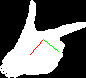
\includegraphics{direction.png}}
\caption{Image segmentée et binarisée d'une main, avec en vert et rouge les deux vecteurs propres de la matrice de covariance.}
\label{fig:pca}
\end{figure}

\subsection{Détection de la direction du pouce}
\subsubsection{Présentation de la méthode}
Un autre problème rencontré est du au mélange de mains gauche et droite dans les données, ainsi que de mains de dos et mains de face. En effet, avec les même doigts levés, ces images n'ont pas les même caractéristiques. Pour ceci, nous estimons la direction des doigts de la main en calculant le décalage horizontal et vertical du centre de gravité de la main avec le centre de la paume de la main. Nous calculons le centre de la paume en supprimant les doigts de l'image binarisée par érosion avec un élément structurant suffisamment grand pour supprimer entièrement les doigts de la main (\autoref{fig:segBinRadialCentres}). Si le décalage est supérieur à un $\epsilon > 0$ fixe, alors nous somme capable de déterminer le "sens" de la main.

\subsubsection{Analyse}
Cette méthode ne permet pas cependant de conclure dans tous les cas, notamment lorsque le décalage entre les centres est trop faible (dans le cas d'une main sans doigts levés, ou sans pouce levé par exemple). Il est alors préférable d'utiliser une méthode de classification invariante par symétrie d'axe vertical comme l'histogramme de projection horizontal.

\begin{figure}[htb!]
\centerline{
\includegraphics{handCenters.png}}
\caption{Image segmentée et binarisée d'une main, avec en vert le centre de la paume de la main et en rouge le centre de gravité de la main.}
\label{fig:segBinRadialCentres}
\end{figure}